\documentclass{standalone}
\usepackage{tikz}
\usetikzlibrary{patterns, positioning}


\begin{document}
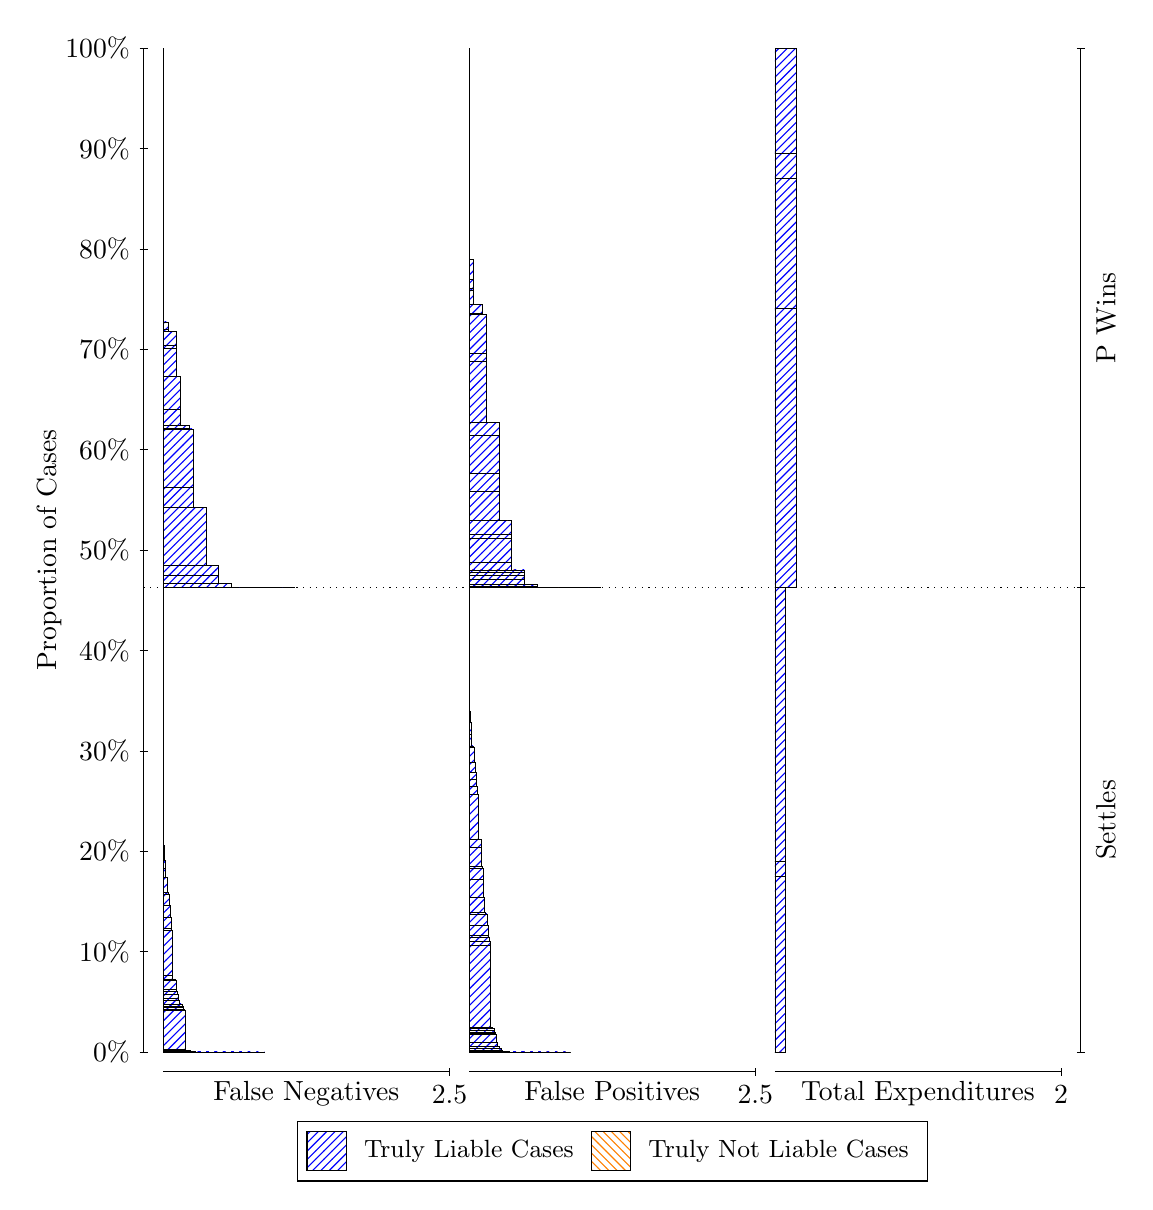
\begin{tikzpicture}
\draw[black, very thin] (1.5,1.75) -- (1.5,14.5);
\node[rotate=90, text=black, anchor=center] at (0.3, 8.125) {Proportion of Cases};
\draw[black, very thin] (1.45,1.75) -- (1.55,1.75);
\node[text=black, anchor=east] at (1.45, 1.75) {0\%};
\draw[black, very thin] (1.45,3.025) -- (1.55,3.025);
\node[text=black, anchor=east] at (1.45, 3.025) {10\%};
\draw[black, very thin] (1.45,4.3) -- (1.55,4.3);
\node[text=black, anchor=east] at (1.45, 4.3) {20\%};
\draw[black, very thin] (1.45,5.575) -- (1.55,5.575);
\node[text=black, anchor=east] at (1.45, 5.575) {30\%};
\draw[black, very thin] (1.45,6.85) -- (1.55,6.85);
\node[text=black, anchor=east] at (1.45, 6.85) {40\%};
\draw[black, very thin] (1.45,8.125) -- (1.55,8.125);
\node[text=black, anchor=east] at (1.45, 8.125) {50\%};
\draw[black, very thin] (1.45,9.4) -- (1.55,9.4);
\node[text=black, anchor=east] at (1.45, 9.4) {60\%};
\draw[black, very thin] (1.45,10.675) -- (1.55,10.675);
\node[text=black, anchor=east] at (1.45, 10.675) {70\%};
\draw[black, very thin] (1.45,11.95) -- (1.55,11.95);
\node[text=black, anchor=east] at (1.45, 11.95) {80\%};
\draw[black, very thin] (1.45,13.225) -- (1.55,13.225);
\node[text=black, anchor=east] at (1.45, 13.225) {90\%};
\draw[black, very thin] (1.45,14.5) -- (1.55,14.5);
\node[text=black, anchor=east] at (1.45, 14.5) {100\%};

\draw[black, very thin] (13.4,1.75) -- (13.4,14.5);
\draw[black, very thin] (13.35,1.75) -- (13.45,1.75);
\node[anchor=west] at (13.35, 1.75) {};
\draw[black, very thin] (13.35,7.6465) -- (13.45,7.6465);
\node[anchor=west] at (13.35, 7.6465) {};
\draw[black, very thin] (13.35,14.5) -- (13.45,14.5);
\node[anchor=west] at (13.35, 14.5) {};

\draw[black, very thin, pattern color=blue, pattern=north east lines] (1.75,1.75) rectangle (3.0398,1.75);
\draw[black, very thin, pattern color=blue, pattern=north east lines] (1.75,1.75) rectangle (2.9672,1.75);
\draw[black, very thin, pattern color=blue, pattern=north east lines] (1.75,1.75) rectangle (2.8945,1.75);
\draw[black, very thin, pattern color=blue, pattern=north east lines] (1.75,1.75) rectangle (2.8784,1.75);
\draw[black, very thin, pattern color=blue, pattern=north east lines] (1.75,1.75) rectangle (2.8218,1.75);
\draw[black, very thin, pattern color=blue, pattern=north east lines] (1.75,1.75) rectangle (2.8057,1.75);
\draw[black, very thin, pattern color=blue, pattern=north east lines] (1.75,1.75) rectangle (2.7492,1.75);
\draw[black, very thin, pattern color=blue, pattern=north east lines] (1.75,1.75) rectangle (2.733,1.75);
\draw[black, very thin, pattern color=blue, pattern=north east lines] (1.75,1.75) rectangle (2.7169,1.75);
\draw[black, very thin, pattern color=blue, pattern=north east lines] (1.75,1.75) rectangle (2.6765,1.75);
\draw[black, very thin, pattern color=blue, pattern=north east lines] (1.75,1.75) rectangle (2.6604,1.75);
\draw[black, very thin, pattern color=blue, pattern=north east lines] (1.75,1.75) rectangle (2.6442,1.75);
\draw[black, very thin, pattern color=blue, pattern=north east lines] (1.75,1.75) rectangle (2.6038,1.75);
\draw[black, very thin, pattern color=blue, pattern=north east lines] (1.75,1.75) rectangle (2.5877,1.75);
\draw[black, very thin, pattern color=blue, pattern=north east lines] (1.75,1.75) rectangle (2.5715,1.75);
\draw[black, very thin, pattern color=blue, pattern=north east lines] (1.75,1.75) rectangle (2.5554,1.75);
\draw[black, very thin, pattern color=blue, pattern=north east lines] (1.75,1.75) rectangle (2.5312,1.75);
\draw[black, very thin, pattern color=blue, pattern=north east lines] (1.75,1.75) rectangle (2.515,1.75);
\draw[black, very thin, pattern color=blue, pattern=north east lines] (1.75,1.75) rectangle (2.4989,1.75);
\draw[black, very thin, pattern color=blue, pattern=north east lines] (1.75,1.75) rectangle (2.4827,1.75);
\draw[black, very thin, pattern color=blue, pattern=north east lines] (1.75,1.75) rectangle (2.4585,1.75);
\draw[black, very thin, pattern color=blue, pattern=north east lines] (1.75,1.75) rectangle (2.4424,1.75);
\draw[black, very thin, pattern color=blue, pattern=north east lines] (1.75,1.75) rectangle (2.4262,1.75);
\draw[black, very thin, pattern color=blue, pattern=north east lines] (1.75,1.75) rectangle (2.4101,1.75);
\draw[black, very thin, pattern color=blue, pattern=north east lines] (1.75,1.75) rectangle (2.3939,1.75);
\draw[black, very thin, pattern color=blue, pattern=north east lines] (1.75,1.75) rectangle (2.3858,1.75);
\draw[black, very thin, pattern color=blue, pattern=north east lines] (1.75,1.75) rectangle (2.3697,1.75);
\draw[black, very thin, pattern color=blue, pattern=north east lines] (1.75,1.75) rectangle (2.3535,1.75);
\draw[black, very thin, pattern color=blue, pattern=north east lines] (1.75,1.75) rectangle (2.3374,1.75);
\draw[black, very thin, pattern color=blue, pattern=north east lines] (1.75,1.75) rectangle (2.3212,1.75);
\draw[black, very thin, pattern color=blue, pattern=north east lines] (1.75,1.75) rectangle (2.3132,1.75);
\draw[black, very thin, pattern color=blue, pattern=north east lines] (1.75,1.75) rectangle (2.297,1.75);
\draw[black, very thin, pattern color=blue, pattern=north east lines] (1.75,1.75) rectangle (2.2809,1.75);
\draw[black, very thin, pattern color=blue, pattern=north east lines] (1.75,1.75) rectangle (2.2647,1.75);
\draw[black, very thin, pattern color=blue, pattern=north east lines] (1.75,1.75) rectangle (2.2486,1.75);
\draw[black, very thin, pattern color=blue, pattern=north east lines] (1.75,1.75) rectangle (2.2405,1.7501);
\draw[black, very thin, pattern color=blue, pattern=north east lines] (1.75,1.7501) rectangle (2.2324,1.7501);
\draw[black, very thin, pattern color=blue, pattern=north east lines] (1.75,1.7501) rectangle (2.2244,1.7501);
\draw[black, very thin, pattern color=blue, pattern=north east lines] (1.75,1.7501) rectangle (2.2082,1.7501);
\draw[black, very thin, pattern color=blue, pattern=north east lines] (1.75,1.7501) rectangle (2.1921,1.7502);
\draw[black, very thin, pattern color=blue, pattern=north east lines] (1.75,1.7502) rectangle (2.1759,1.7504);
\draw[black, very thin, pattern color=blue, pattern=north east lines] (1.75,1.7504) rectangle (2.1678,1.7518);
\draw[black, very thin, pattern color=blue, pattern=north east lines] (1.75,1.7518) rectangle (2.1598,1.7522);
\draw[black, very thin, pattern color=blue, pattern=north east lines] (1.75,1.7522) rectangle (2.1517,1.7528);
\draw[black, very thin, pattern color=blue, pattern=north east lines] (1.75,1.7528) rectangle (2.1355,1.7529);
\draw[black, very thin, pattern color=blue, pattern=north east lines] (1.75,1.7529) rectangle (2.1194,1.7552);
\draw[black, very thin, pattern color=blue, pattern=north east lines] (1.75,1.7552) rectangle (2.1032,1.7556);
\draw[black, very thin, pattern color=blue, pattern=north east lines] (1.75,1.7556) rectangle (2.0952,1.7656);
\draw[black, very thin, pattern color=blue, pattern=north east lines] (1.75,1.7656) rectangle (2.0871,1.7675);
\draw[black, very thin, pattern color=blue, pattern=north east lines] (1.75,1.7675) rectangle (2.079,1.7697);
\draw[black, very thin, pattern color=blue, pattern=north east lines] (1.75,1.7697) rectangle (2.0709,1.7754);
\draw[black, very thin, pattern color=blue, pattern=north east lines] (1.75,1.7754) rectangle (2.0629,1.7755);
\draw[black, very thin, pattern color=blue, pattern=north east lines] (1.75,1.7755) rectangle (2.0467,1.7756);
\draw[black, very thin, pattern color=blue, pattern=north east lines] (1.75,1.7756) rectangle (2.0306,1.7804);
\draw[black, very thin, pattern color=blue, pattern=north east lines] (1.75,1.7804) rectangle (2.0225,2.284);
\draw[black, very thin, pattern color=blue, pattern=north east lines] (1.75,2.284) rectangle (2.0144,2.289);
\draw[black, very thin, pattern color=blue, pattern=north east lines] (1.75,2.289) rectangle (2.0064,2.3161);
\draw[black, very thin, pattern color=blue, pattern=north east lines] (1.75,2.3161) rectangle (1.9983,2.3366);
\draw[black, very thin, pattern color=blue, pattern=north east lines] (1.75,2.3366) rectangle (1.9902,2.3575);
\draw[black, very thin, pattern color=blue, pattern=north east lines] (1.75,2.3575) rectangle (1.9741,2.3605);
\draw[black, very thin, pattern color=blue, pattern=north east lines] (1.75,2.3605) rectangle (1.9579,2.4088);
\draw[black, very thin, pattern color=blue, pattern=north east lines] (1.75,2.4088) rectangle (1.9418,2.4275);
\draw[black, very thin, pattern color=blue, pattern=north east lines] (1.75,2.4275) rectangle (1.9337,2.4829);
\draw[black, very thin, pattern color=blue, pattern=north east lines] (1.75,2.4829) rectangle (1.9256,2.5154);
\draw[black, very thin, pattern color=blue, pattern=north east lines] (1.75,2.5154) rectangle (1.9175,2.5483);
\draw[black, very thin, pattern color=blue, pattern=north east lines] (1.75,2.5483) rectangle (1.9095,2.6663);
\draw[black, very thin, pattern color=blue, pattern=north east lines] (1.75,2.6663) rectangle (1.9014,2.6682);
\draw[black, very thin, pattern color=blue, pattern=north east lines] (1.75,2.6682) rectangle (1.8852,2.67);
\draw[black, very thin, pattern color=blue, pattern=north east lines] (1.75,2.67) rectangle (1.8691,2.7188);
\draw[black, very thin, pattern color=blue, pattern=north east lines] (1.75,2.7188) rectangle (1.861,3.2901);
\draw[black, very thin, pattern color=blue, pattern=north east lines] (1.75,3.2901) rectangle (1.8529,3.3157);
\draw[black, very thin, pattern color=blue, pattern=north east lines] (1.75,3.3157) rectangle (1.8449,3.4612);
\draw[black, very thin, pattern color=blue, pattern=north east lines] (1.75,3.4612) rectangle (1.8368,3.6107);
\draw[black, very thin, pattern color=blue, pattern=north east lines] (1.75,3.6107) rectangle (1.8287,3.7588);
\draw[black, very thin, pattern color=blue, pattern=north east lines] (1.75,3.7588) rectangle (1.8126,3.778);
\draw[black, very thin, pattern color=blue, pattern=north east lines] (1.75,3.778) rectangle (1.7964,3.9706);
\draw[black, very thin, pattern color=blue, pattern=north east lines] (1.75,3.9706) rectangle (1.7803,4.0886);
\draw[black, very thin, pattern color=blue, pattern=north east lines] (1.75,4.0886) rectangle (1.7722,4.183);
\draw[black, very thin, pattern color=blue, pattern=north east lines] (1.75,4.183) rectangle (1.7641,4.2773);
\draw[black, very thin, pattern color=blue, pattern=north east lines] (1.75,4.2773) rectangle (1.7561,4.3705);
\draw[black, very thin, pattern color=orange, pattern=north west lines] (1.75,4.3705) rectangle (1.75,4.3705);
\draw[black, very thin, pattern color=blue, pattern=north east lines] (1.75,4.3705) rectangle (1.75,7.6465);
\draw[black, very thin, pattern color=blue, pattern=north east lines] (1.75,7.6465) rectangle (3.4213,7.6465);
\draw[black, very thin, pattern color=blue, pattern=north east lines] (1.75,7.6465) rectangle (3.2599,7.6465);
\draw[black, very thin, pattern color=blue, pattern=north east lines] (1.75,7.6465) rectangle (3.2599,7.6465);
\draw[black, very thin, pattern color=blue, pattern=north east lines] (1.75,7.6465) rectangle (3.0984,7.6465);
\draw[black, very thin, pattern color=blue, pattern=north east lines] (1.75,7.6465) rectangle (3.0984,7.6465);
\draw[black, very thin, pattern color=blue, pattern=north east lines] (1.75,7.6465) rectangle (2.9369,7.6469);
\draw[black, very thin, pattern color=blue, pattern=north east lines] (1.75,7.6469) rectangle (2.8804,7.6469);
\draw[black, very thin, pattern color=blue, pattern=north east lines] (1.75,7.6469) rectangle (2.7754,7.6505);
\draw[black, very thin, pattern color=blue, pattern=north east lines] (1.75,7.6505) rectangle (2.7754,7.6524);
\draw[black, very thin, pattern color=blue, pattern=north east lines] (1.75,7.6524) rectangle (2.7189,7.6524);
\draw[black, very thin, pattern color=blue, pattern=north east lines] (1.75,7.6524) rectangle (2.7189,7.6524);
\draw[black, very thin, pattern color=blue, pattern=north east lines] (1.75,7.6524) rectangle (2.6139,7.6982);
\draw[black, very thin, pattern color=blue, pattern=north east lines] (1.75,7.6982) rectangle (2.5574,7.6982);
\draw[black, very thin, pattern color=blue, pattern=north east lines] (1.75,7.6982) rectangle (2.4524,7.8079);
\draw[black, very thin, pattern color=blue, pattern=north east lines] (1.75,7.8079) rectangle (2.4524,7.934);
\draw[black, very thin, pattern color=blue, pattern=north east lines] (1.75,7.934) rectangle (2.3959,7.934);
\draw[black, very thin, pattern color=blue, pattern=north east lines] (1.75,7.934) rectangle (2.3959,7.934);
\draw[black, very thin, pattern color=blue, pattern=north east lines] (1.75,7.934) rectangle (2.291,8.6626);
\draw[black, very thin, pattern color=blue, pattern=north east lines] (1.75,8.6626) rectangle (2.2344,8.6633);
\draw[black, very thin, pattern color=blue, pattern=north east lines] (1.75,8.6633) rectangle (2.2344,8.6633);
\draw[black, very thin, pattern color=blue, pattern=north east lines] (1.75,8.6633) rectangle (2.2344,8.6637);
\draw[black, very thin, pattern color=blue, pattern=north east lines] (1.75,8.6637) rectangle (2.1295,8.922);
\draw[black, very thin, pattern color=blue, pattern=north east lines] (1.75,8.922) rectangle (2.1295,9.6637);
\draw[black, very thin, pattern color=blue, pattern=north east lines] (1.75,9.6637) rectangle (2.073,9.6646);
\draw[black, very thin, pattern color=blue, pattern=north east lines] (1.75,9.6646) rectangle (2.073,9.7098);
\draw[black, very thin, pattern color=blue, pattern=north east lines] (1.75,9.7098) rectangle (1.968,9.913);
\draw[black, very thin, pattern color=blue, pattern=north east lines] (1.75,9.913) rectangle (1.968,10.329);
\draw[black, very thin, pattern color=blue, pattern=north east lines] (1.75,10.329) rectangle (1.9115,10.684);
\draw[black, very thin, pattern color=blue, pattern=north east lines] (1.75,10.684) rectangle (1.9115,10.719);
\draw[black, very thin, pattern color=blue, pattern=north east lines] (1.75,10.719) rectangle (1.9115,10.902);
\draw[black, very thin, pattern color=blue, pattern=north east lines] (1.75,10.902) rectangle (1.8065,10.903);
\draw[black, very thin, pattern color=blue, pattern=north east lines] (1.75,10.903) rectangle (1.8065,10.928);
\draw[black, very thin, pattern color=blue, pattern=north east lines] (1.75,10.928) rectangle (1.8065,11.02);
\draw[black, very thin, pattern color=blue, pattern=north east lines] (1.75,11.02) rectangle (1.8065,11.022);
\draw[black, very thin, pattern color=orange, pattern=north west lines] (1.75,11.022) rectangle (1.75,11.022);
\draw[black, very thin, pattern color=blue, pattern=north east lines] (1.75,11.022) rectangle (1.75,14.5);
\draw[black, very thin, pattern color=orange, pattern=north west lines] (5.6333,1.75) rectangle (6.9232,1.75);
\draw[black, very thin, pattern color=blue, pattern=north east lines] (5.6333,1.75) rectangle (6.9232,1.75);
\draw[black, very thin, pattern color=orange, pattern=north west lines] (5.6333,1.75) rectangle (6.8505,1.75);
\draw[black, very thin, pattern color=blue, pattern=north east lines] (5.6333,1.75) rectangle (6.8505,1.75);
\draw[black, very thin, pattern color=orange, pattern=north west lines] (5.6333,1.75) rectangle (6.7778,1.75);
\draw[black, very thin, pattern color=blue, pattern=north east lines] (5.6333,1.75) rectangle (6.7778,1.75);
\draw[black, very thin, pattern color=blue, pattern=north east lines] (5.6333,1.75) rectangle (6.7617,1.75);
\draw[black, very thin, pattern color=orange, pattern=north west lines] (5.6333,1.75) rectangle (6.7052,1.75);
\draw[black, very thin, pattern color=blue, pattern=north east lines] (5.6333,1.75) rectangle (6.7052,1.75);
\draw[black, very thin, pattern color=blue, pattern=north east lines] (5.6333,1.75) rectangle (6.689,1.75);
\draw[black, very thin, pattern color=orange, pattern=north west lines] (5.6333,1.75) rectangle (6.6325,1.75);
\draw[black, very thin, pattern color=blue, pattern=north east lines] (5.6333,1.75) rectangle (6.6325,1.75);
\draw[black, very thin, pattern color=blue, pattern=north east lines] (5.6333,1.75) rectangle (6.6164,1.75);
\draw[black, very thin, pattern color=blue, pattern=north east lines] (5.6333,1.75) rectangle (6.6002,1.75);
\draw[black, very thin, pattern color=orange, pattern=north west lines] (5.6333,1.75) rectangle (6.5598,1.75);
\draw[black, very thin, pattern color=blue, pattern=north east lines] (5.6333,1.75) rectangle (6.5598,1.75);
\draw[black, very thin, pattern color=blue, pattern=north east lines] (5.6333,1.75) rectangle (6.5437,1.75);
\draw[black, very thin, pattern color=blue, pattern=north east lines] (5.6333,1.75) rectangle (6.5275,1.75);
\draw[black, very thin, pattern color=orange, pattern=north west lines] (5.6333,1.75) rectangle (6.4872,1.75);
\draw[black, very thin, pattern color=blue, pattern=north east lines] (5.6333,1.75) rectangle (6.4872,1.75);
\draw[black, very thin, pattern color=blue, pattern=north east lines] (5.6333,1.75) rectangle (6.471,1.75);
\draw[black, very thin, pattern color=blue, pattern=north east lines] (5.6333,1.75) rectangle (6.4549,1.75);
\draw[black, very thin, pattern color=blue, pattern=north east lines] (5.6333,1.75) rectangle (6.4387,1.75);
\draw[black, very thin, pattern color=orange, pattern=north west lines] (5.6333,1.75) rectangle (6.4145,1.75);
\draw[black, very thin, pattern color=blue, pattern=north east lines] (5.6333,1.75) rectangle (6.4145,1.75);
\draw[black, very thin, pattern color=blue, pattern=north east lines] (5.6333,1.75) rectangle (6.3984,1.75);
\draw[black, very thin, pattern color=blue, pattern=north east lines] (5.6333,1.75) rectangle (6.3822,1.75);
\draw[black, very thin, pattern color=blue, pattern=north east lines] (5.6333,1.75) rectangle (6.3661,1.75);
\draw[black, very thin, pattern color=orange, pattern=north west lines] (5.6333,1.75) rectangle (6.3418,1.75);
\draw[black, very thin, pattern color=blue, pattern=north east lines] (5.6333,1.75) rectangle (6.3418,1.75);
\draw[black, very thin, pattern color=blue, pattern=north east lines] (5.6333,1.75) rectangle (6.3257,1.75);
\draw[black, very thin, pattern color=blue, pattern=north east lines] (5.6333,1.75) rectangle (6.3095,1.75);
\draw[black, very thin, pattern color=blue, pattern=north east lines] (5.6333,1.75) rectangle (6.2934,1.75);
\draw[black, very thin, pattern color=blue, pattern=north east lines] (5.6333,1.75) rectangle (6.2772,1.75);
\draw[black, very thin, pattern color=orange, pattern=north west lines] (5.6333,1.75) rectangle (6.2692,1.75);
\draw[black, very thin, pattern color=blue, pattern=north east lines] (5.6333,1.75) rectangle (6.2692,1.7501);
\draw[black, very thin, pattern color=blue, pattern=north east lines] (5.6333,1.7501) rectangle (6.253,1.7501);
\draw[black, very thin, pattern color=blue, pattern=north east lines] (5.6333,1.7501) rectangle (6.2369,1.7501);
\draw[black, very thin, pattern color=blue, pattern=north east lines] (5.6333,1.7501) rectangle (6.2207,1.7502);
\draw[black, very thin, pattern color=blue, pattern=north east lines] (5.6333,1.7502) rectangle (6.2046,1.7502);
\draw[black, very thin, pattern color=orange, pattern=north west lines] (5.6333,1.7502) rectangle (6.1965,1.7502);
\draw[black, very thin, pattern color=blue, pattern=north east lines] (5.6333,1.7502) rectangle (6.1965,1.7511);
\draw[black, very thin, pattern color=blue, pattern=north east lines] (5.6333,1.7511) rectangle (6.1804,1.7517);
\draw[black, very thin, pattern color=blue, pattern=north east lines] (5.6333,1.7517) rectangle (6.1642,1.7518);
\draw[black, very thin, pattern color=blue, pattern=north east lines] (5.6333,1.7518) rectangle (6.1481,1.7541);
\draw[black, very thin, pattern color=blue, pattern=north east lines] (5.6333,1.7541) rectangle (6.1319,1.7547);
\draw[black, very thin, pattern color=orange, pattern=north west lines] (5.6333,1.7547) rectangle (6.1238,1.7547);
\draw[black, very thin, pattern color=blue, pattern=north east lines] (5.6333,1.7547) rectangle (6.1238,1.7551);
\draw[black, very thin, pattern color=blue, pattern=north east lines] (5.6333,1.7551) rectangle (6.1158,1.7556);
\draw[black, very thin, pattern color=blue, pattern=north east lines] (5.6333,1.7556) rectangle (6.1077,1.7578);
\draw[black, very thin, pattern color=blue, pattern=north east lines] (5.6333,1.7578) rectangle (6.0915,1.7579);
\draw[black, very thin, pattern color=blue, pattern=north east lines] (5.6333,1.7579) rectangle (6.0754,1.7581);
\draw[black, very thin, pattern color=blue, pattern=north east lines] (5.6333,1.7581) rectangle (6.0592,1.7628);
\draw[black, very thin, pattern color=orange, pattern=north west lines] (5.6333,1.7628) rectangle (6.0512,1.7628);
\draw[black, very thin, pattern color=blue, pattern=north east lines] (5.6333,1.7628) rectangle (6.0512,1.7728);
\draw[black, very thin, pattern color=blue, pattern=north east lines] (5.6333,1.7728) rectangle (6.0431,1.7747);
\draw[black, very thin, pattern color=blue, pattern=north east lines] (5.6333,1.7747) rectangle (6.035,1.7961);
\draw[black, very thin, pattern color=blue, pattern=north east lines] (5.6333,1.7961) rectangle (6.0189,1.8169);
\draw[black, very thin, pattern color=blue, pattern=north east lines] (5.6333,1.8169) rectangle (6.0027,1.8199);
\draw[black, very thin, pattern color=blue, pattern=north east lines] (5.6333,1.8199) rectangle (5.9866,1.8682);
\draw[black, very thin, pattern color=orange, pattern=north west lines] (5.6333,1.8682) rectangle (5.9785,1.8682);
\draw[black, very thin, pattern color=blue, pattern=north east lines] (5.6333,1.8682) rectangle (5.9785,1.9692);
\draw[black, very thin, pattern color=blue, pattern=north east lines] (5.6333,1.9692) rectangle (5.9704,1.9928);
\draw[black, very thin, pattern color=blue, pattern=north east lines] (5.6333,1.9928) rectangle (5.9624,1.9985);
\draw[black, very thin, pattern color=blue, pattern=north east lines] (5.6333,1.9985) rectangle (5.9543,2.0241);
\draw[black, very thin, pattern color=blue, pattern=north east lines] (5.6333,2.0241) rectangle (5.9462,2.0571);
\draw[black, very thin, pattern color=blue, pattern=north east lines] (5.6333,2.0571) rectangle (5.9301,2.059);
\draw[black, very thin, pattern color=blue, pattern=north east lines] (5.6333,2.059) rectangle (5.9139,2.0608);
\draw[black, very thin, pattern color=orange, pattern=north west lines] (5.6333,2.0608) rectangle (5.9058,2.0608);
\draw[black, very thin, pattern color=blue, pattern=north east lines] (5.6333,2.0608) rectangle (5.9058,3.1014);
\draw[black, very thin, pattern color=blue, pattern=north east lines] (5.6333,3.1014) rectangle (5.8978,3.1496);
\draw[black, very thin, pattern color=blue, pattern=north east lines] (5.6333,3.1496) rectangle (5.8897,3.205);
\draw[black, very thin, pattern color=blue, pattern=north east lines] (5.6333,3.205) rectangle (5.8816,3.2376);
\draw[black, very thin, pattern color=blue, pattern=north east lines] (5.6333,3.2376) rectangle (5.8735,3.3571);
\draw[black, very thin, pattern color=blue, pattern=north east lines] (5.6333,3.3571) rectangle (5.8574,3.5048);
\draw[black, very thin, pattern color=blue, pattern=north east lines] (5.6333,3.5048) rectangle (5.8412,3.5239);
\draw[black, very thin, pattern color=blue, pattern=north east lines] (5.6333,3.5239) rectangle (5.8251,3.7169);
\draw[black, very thin, pattern color=blue, pattern=north east lines] (5.6333,3.7169) rectangle (5.817,3.938);
\draw[black, very thin, pattern color=blue, pattern=north east lines] (5.6333,3.938) rectangle (5.8089,4.0817);
\draw[black, very thin, pattern color=blue, pattern=north east lines] (5.6333,4.0817) rectangle (5.8009,4.1077);
\draw[black, very thin, pattern color=blue, pattern=north east lines] (5.6333,4.1077) rectangle (5.7928,4.3515);
\draw[black, very thin, pattern color=blue, pattern=north east lines] (5.6333,4.3515) rectangle (5.7847,4.4452);
\draw[black, very thin, pattern color=blue, pattern=north east lines] (5.6333,4.4452) rectangle (5.7686,4.4499);
\draw[black, very thin, pattern color=blue, pattern=north east lines] (5.6333,4.4499) rectangle (5.7524,4.4547);
\draw[black, very thin, pattern color=blue, pattern=north east lines] (5.6333,4.4547) rectangle (5.7444,5.0259);
\draw[black, very thin, pattern color=blue, pattern=north east lines] (5.6333,5.0259) rectangle (5.7363,5.1192);
\draw[black, very thin, pattern color=blue, pattern=north east lines] (5.6333,5.1192) rectangle (5.7282,5.2135);
\draw[black, very thin, pattern color=blue, pattern=north east lines] (5.6333,5.2135) rectangle (5.7201,5.3078);
\draw[black, very thin, pattern color=blue, pattern=north east lines] (5.6333,5.3078) rectangle (5.7121,5.4259);
\draw[black, very thin, pattern color=blue, pattern=north east lines] (5.6333,5.4259) rectangle (5.6959,5.6185);
\draw[black, very thin, pattern color=blue, pattern=north east lines] (5.6333,5.6185) rectangle (5.6798,5.6376);
\draw[black, very thin, pattern color=blue, pattern=north east lines] (5.6333,5.6376) rectangle (5.6636,5.7858);
\draw[black, very thin, pattern color=blue, pattern=north east lines] (5.6333,5.7858) rectangle (5.6555,5.9353);
\draw[black, very thin, pattern color=blue, pattern=north east lines] (5.6333,5.9353) rectangle (5.6475,6.0807);
\draw[black, very thin, pattern color=blue, pattern=north east lines] (5.6333,6.0807) rectangle (5.6394,6.1064);
\draw[black, very thin, pattern color=blue, pattern=north east lines] (5.6333,6.1064) rectangle (5.6333,7.6465);
\draw[black, very thin, pattern color=orange, pattern=north west lines] (5.6333,7.6465) rectangle (7.3047,7.6465);
\draw[black, very thin, pattern color=blue, pattern=north east lines] (5.6333,7.6465) rectangle (7.3047,7.6465);
\draw[black, very thin, pattern color=orange, pattern=north west lines] (5.6333,7.6465) rectangle (7.1432,7.6465);
\draw[black, very thin, pattern color=blue, pattern=north east lines] (5.6333,7.6465) rectangle (7.1432,7.6465);
\draw[black, very thin, pattern color=orange, pattern=north west lines] (5.6333,7.6465) rectangle (6.9817,7.6465);
\draw[black, very thin, pattern color=blue, pattern=north east lines] (5.6333,7.6465) rectangle (6.9817,7.6465);
\draw[black, very thin, pattern color=blue, pattern=north east lines] (5.6333,7.6465) rectangle (6.9817,7.6465);
\draw[black, very thin, pattern color=blue, pattern=north east lines] (5.6333,7.6465) rectangle (6.9817,7.6465);
\draw[black, very thin, pattern color=orange, pattern=north west lines] (5.6333,7.6465) rectangle (6.8202,7.6465);
\draw[black, very thin, pattern color=blue, pattern=north east lines] (5.6333,7.6465) rectangle (6.8202,7.6467);
\draw[black, very thin, pattern color=blue, pattern=north east lines] (5.6333,7.6467) rectangle (6.8202,7.6467);
\draw[black, very thin, pattern color=orange, pattern=north west lines] (5.6333,7.6467) rectangle (6.7637,7.6467);
\draw[black, very thin, pattern color=blue, pattern=north east lines] (5.6333,7.6467) rectangle (6.7637,7.6467);
\draw[black, very thin, pattern color=orange, pattern=north west lines] (5.6333,7.6467) rectangle (6.6587,7.6467);
\draw[black, very thin, pattern color=blue, pattern=north east lines] (5.6333,7.6467) rectangle (6.6587,7.6479);
\draw[black, very thin, pattern color=blue, pattern=north east lines] (5.6333,7.6479) rectangle (6.6587,7.6506);
\draw[black, very thin, pattern color=blue, pattern=north east lines] (5.6333,7.6506) rectangle (6.6022,7.6506);
\draw[black, very thin, pattern color=orange, pattern=north west lines] (5.6333,7.6506) rectangle (6.6022,7.6506);
\draw[black, very thin, pattern color=blue, pattern=north east lines] (5.6333,7.6506) rectangle (6.6022,7.6506);
\draw[black, very thin, pattern color=blue, pattern=north east lines] (5.6333,7.6506) rectangle (6.4973,7.6617);
\draw[black, very thin, pattern color=orange, pattern=north west lines] (5.6333,7.6617) rectangle (6.4973,7.6617);
\draw[black, very thin, pattern color=blue, pattern=north east lines] (5.6333,7.6617) rectangle (6.4973,7.6697);
\draw[black, very thin, pattern color=blue, pattern=north east lines] (5.6333,7.6697) rectangle (6.4973,7.6854);
\draw[black, very thin, pattern color=orange, pattern=north west lines] (5.6333,7.6854) rectangle (6.4407,7.6854);
\draw[black, very thin, pattern color=blue, pattern=north east lines] (5.6333,7.6854) rectangle (6.4407,7.6854);
\draw[black, very thin, pattern color=blue, pattern=north east lines] (5.6333,7.6854) rectangle (6.3358,7.7492);
\draw[black, very thin, pattern color=blue, pattern=north east lines] (5.6333,7.7492) rectangle (6.3358,7.7987);
\draw[black, very thin, pattern color=orange, pattern=north west lines] (5.6333,7.7987) rectangle (6.3358,7.7987);
\draw[black, very thin, pattern color=blue, pattern=north east lines] (5.6333,7.7987) rectangle (6.3358,7.8377);
\draw[black, very thin, pattern color=blue, pattern=north east lines] (5.6333,7.8377) rectangle (6.3358,7.873);
\draw[black, very thin, pattern color=blue, pattern=north east lines] (5.6333,7.873) rectangle (6.2793,7.873);
\draw[black, very thin, pattern color=orange, pattern=north west lines] (5.6333,7.873) rectangle (6.2793,7.873);
\draw[black, very thin, pattern color=blue, pattern=north east lines] (5.6333,7.873) rectangle (6.2793,7.873);
\draw[black, very thin, pattern color=blue, pattern=north east lines] (5.6333,7.873) rectangle (6.1743,7.9652);
\draw[black, very thin, pattern color=orange, pattern=north west lines] (5.6333,7.9652) rectangle (6.1743,7.9652);
\draw[black, very thin, pattern color=blue, pattern=north east lines] (5.6333,7.9652) rectangle (6.1743,8.2733);
\draw[black, very thin, pattern color=blue, pattern=north east lines] (5.6333,8.2733) rectangle (6.1743,8.3249);
\draw[black, very thin, pattern color=blue, pattern=north east lines] (5.6333,8.3249) rectangle (6.1743,8.503);
\draw[black, very thin, pattern color=blue, pattern=north east lines] (5.6333,8.503) rectangle (6.1178,8.503);
\draw[black, very thin, pattern color=orange, pattern=north west lines] (5.6333,8.503) rectangle (6.1178,8.503);
\draw[black, very thin, pattern color=blue, pattern=north east lines] (5.6333,8.503) rectangle (6.1178,8.503);
\draw[black, very thin, pattern color=blue, pattern=north east lines] (5.6333,8.503) rectangle (6.0128,8.8732);
\draw[black, very thin, pattern color=blue, pattern=north east lines] (5.6333,8.8732) rectangle (6.0128,9.0939);
\draw[black, very thin, pattern color=blue, pattern=north east lines] (5.6333,9.0939) rectangle (6.0128,9.5791);
\draw[black, very thin, pattern color=blue, pattern=north east lines] (5.6333,9.5791) rectangle (6.0128,9.7424);
\draw[black, very thin, pattern color=blue, pattern=north east lines] (5.6333,9.7424) rectangle (5.9563,9.7424);
\draw[black, very thin, pattern color=orange, pattern=north west lines] (5.6333,9.7424) rectangle (5.9563,9.7424);
\draw[black, very thin, pattern color=blue, pattern=north east lines] (5.6333,9.7424) rectangle (5.9563,9.7457);
\draw[black, very thin, pattern color=blue, pattern=north east lines] (5.6333,9.7457) rectangle (5.8513,10.521);
\draw[black, very thin, pattern color=blue, pattern=north east lines] (5.6333,10.521) rectangle (5.8513,10.618);
\draw[black, very thin, pattern color=blue, pattern=north east lines] (5.6333,10.618) rectangle (5.8513,11.125);
\draw[black, very thin, pattern color=blue, pattern=north east lines] (5.6333,11.125) rectangle (5.7948,11.126);
\draw[black, very thin, pattern color=orange, pattern=north west lines] (5.6333,11.126) rectangle (5.7948,11.126);
\draw[black, very thin, pattern color=blue, pattern=north east lines] (5.6333,11.126) rectangle (5.7948,11.244);
\draw[black, very thin, pattern color=blue, pattern=north east lines] (5.6333,11.244) rectangle (5.7948,11.245);
\draw[black, very thin, pattern color=blue, pattern=north east lines] (5.6333,11.245) rectangle (5.6899,11.428);
\draw[black, very thin, pattern color=blue, pattern=north east lines] (5.6333,11.428) rectangle (5.6899,11.445);
\draw[black, very thin, pattern color=blue, pattern=north east lines] (5.6333,11.445) rectangle (5.6899,11.563);
\draw[black, very thin, pattern color=blue, pattern=north east lines] (5.6333,11.563) rectangle (5.6899,11.817);
\draw[black, very thin, pattern color=orange, pattern=north west lines] (5.6333,11.817) rectangle (5.6333,11.817);
\draw[black, very thin, pattern color=blue, pattern=north east lines] (5.6333,11.817) rectangle (5.6333,14.5);
\draw[black, very thin, pattern color=orange, pattern=north west lines] (9.5167,1.75) rectangle (9.6529,1.75);
\draw[black, very thin, pattern color=blue, pattern=north east lines] (9.5167,1.75) rectangle (9.6529,3.978);
\draw[black, very thin, pattern color=orange, pattern=north west lines] (9.5167,3.978) rectangle (9.6529,3.978);
\draw[black, very thin, pattern color=blue, pattern=north east lines] (9.5167,3.978) rectangle (9.6529,4.1722);
\draw[black, very thin, pattern color=orange, pattern=north west lines] (9.5167,4.1722) rectangle (9.6529,4.1722);
\draw[black, very thin, pattern color=blue, pattern=north east lines] (9.5167,4.1722) rectangle (9.6529,7.6465);
\draw[black, very thin, pattern color=orange, pattern=north west lines] (9.5167,7.6465) rectangle (9.7892,7.6465);
\draw[black, very thin, pattern color=blue, pattern=north east lines] (9.5167,7.6465) rectangle (9.7892,11.196);
\draw[black, very thin, pattern color=orange, pattern=north west lines] (9.5167,11.196) rectangle (9.7892,11.196);
\draw[black, very thin, pattern color=blue, pattern=north east lines] (9.5167,11.196) rectangle (9.7892,12.848);
\draw[black, very thin, pattern color=orange, pattern=north west lines] (9.5167,12.848) rectangle (9.7892,12.848);
\draw[black, very thin, pattern color=blue, pattern=north east lines] (9.5167,12.848) rectangle (9.7892,13.158);
\draw[black, very thin, pattern color=orange, pattern=north west lines] (9.5167,13.158) rectangle (9.7892,13.158);
\draw[black, very thin, pattern color=blue, pattern=north east lines] (9.5167,13.158) rectangle (9.7892,14.5);
\draw[black, dotted] (1.5,7.6465) -- (13.4,7.6465);
\draw[black, very thin] (1.75,1.5) -- (5.3833,1.5);
\node[text=black, anchor=north] at (3.5667, 1.5) {False Negatives};
\draw[black, very thin] (5.3833,1.45) -- (5.3833,1.55);
\node[text=black, anchor=north] at (5.3833, 1.45) {2.5};

\draw[black, very thin] (5.6333,1.5) -- (9.2667,1.5);
\node[text=black, anchor=north] at (7.45, 1.5) {False Positives};
\draw[black, very thin] (9.2667,1.45) -- (9.2667,1.55);
\node[text=black, anchor=north] at (9.2667, 1.45) {2.5};

\draw[black, very thin] (9.5167,1.5) -- (13.15,1.5);
\node[text=black, anchor=north] at (11.333, 1.5) {Total Expenditures};
\draw[black, very thin] (13.15,1.45) -- (13.15,1.55);
\node[text=black, anchor=north] at (13.15, 1.45) {2};

\node[text=black, centered, rotate=90] at (13.72, 4.6982) {Settles};
\node[text=black, centered, rotate=90] at (13.72, 11.073) {P Wins};

\draw (7.449999999999999,1.5) node[draw=none] (baseCoordinate) {};
\begin{scope}[align=center]
        \matrix[scale=0.5, draw=black, below=0.5cm of baseCoordinate, nodes={draw}, column sep=0.1cm]{
            \node[rectangle, draw, minimum width=0.5cm, minimum height=0.5cm, pattern color=blue, pattern=north east lines] {}; &
            \node[draw=none, font=\small, text=black] (B) {Truly Liable Cases}; &
            \node[rectangle, draw, minimum width=0.5cm, minimum height=0.5cm, pattern color=orange, pattern=north west lines] {}; &
            \node[draw=none, font=\small, text=black] (B) {Truly Not Liable Cases}; \\
            };
\end{scope}

\end{tikzpicture}
\end{document}